\documentclass[../../main.tex]{subfiles}
\begin{document}
\begin{oframed}
  \subfile{problem}
\end{oframed}

{\bf [解答]}

\begin{figure}[htbp]
  \centering
  \begin{tikzpicture}[x=1.3cm, y=1.3cm, >=stealth,
    every node/.style={font=\small}]
    \coordinate (O) at (0,-0.2);
    \coordinate (A) at (1.2,3.4);
    \coordinate (B) at (-1.6,1.4);
    \coordinate (C) at (3.2,1.6);
    \coordinate (P) at (1.0,2.0);

    % Face ABC shading
    \fill[teal!12] (A) -- (B) -- (C) -- cycle;

    % Incircle in perspective inside triangle ABC
    \draw[teal!60!black, thin] (P) circle [x radius=0.85cm, y radius=0.48cm, rotate=5];

    % Vectors from O to vertices
    \draw[line width=1.1pt, gray!60, ->] (O) -- (A) node[pos=0.85, left=2pt] {$\overrightarrow{OA}$};
    \draw[line width=1.1pt, gray!75!black, ->] (O) -- (B) node[midway, below left=1pt] {$\overrightarrow{OB}$};
    \draw[line width=1.1pt, gray!75!black, ->] (O) -- (C) node[midway, below right=1pt] {$\overrightarrow{OC}$};

    % Triangle ABC edges
    \draw[line width=1.3pt, teal!75!black] (A) -- (B) -- (C) -- cycle;

    % Angle bisectors to incenter P
    \draw[dashed, teal!65!black] (A) -- (P);
    \draw[dashed, teal!65!black] (B) -- (P);
    \draw[dashed, teal!65!black] (C) -- (P);

    % Vector OP
    \draw[line width=1.4pt, red!85!black, ->] (O) -- (P) node[pos=0.45, right=2pt] {$\overrightarrow{OP}$};

    % Vertices and points
    \foreach \T in {O,A,B,C} {
      \node[circle, fill=blue!85!black, inner sep=1.5pt] at (\T) {};
    }
    \node[circle, fill=red!85!black, inner sep=1.6pt] at (P) {};

    \node[below=2pt] at (O) {$O$};
    \node[above=2pt] at (A) {$A$};
    \node[left=2pt] at (B) {$B$};
    \node[right=2pt] at (C) {$C$};
    \node[above right=1pt, red!85!black] at (P) {$P$};
    \node[below=2pt, teal!80!black] at ($(B)!0.8!(C)$) {$a$};
    \node[above right=2pt, teal!80!black] at ($(A)!0.5!(C)$) {$b$};
    \node[above left=2pt, teal!80!black] at ($(A)!0.5!(B)$) {$c$};
  \end{tikzpicture}
  \caption{空間内の原点 $O$ と三角形 $ABC$ およびその内心 $P$}
  \label{fig:tetrahedron_incenter}
\end{figure}

\paragraph{(1)}

与えられた関係式
\begin{align}
  u\overrightarrow{OA}+v\overrightarrow{OB}+w\overrightarrow{OC}=\vec{0} \label{eq:1}
\end{align}
の左辺を整理すると
\begin{align}
  (\text{左辺})
  & = v \overrightarrow{AB} + w \overrightarrow{AC} + (u+v+w) \overrightarrow{OA}
\end{align}
である．$\overrightarrow{OA}, \overrightarrow{OB}, \overrightarrow{OC}$ はどの2つも平行でないから，$u+v+w \neq 0$の時\cref{eq:1}の左辺の表す点$O'$は$O$と異なる平面にあり不適である．
よって$u+v+w = 0$ だから\cref{eq:1}に代入して
\begin{align}
  v \overrightarrow{AB} + w \overrightarrow{AC} = 0 \label{eq:2}
\end{align}
となる場合を考える．$A,B,C$の張る平面内に$xy$座標をとって
$\overrightarrow{AB} =
\begin{pmatrix} x_1 \\ y_1
\end{pmatrix}, \overrightarrow{AC} =
\begin{pmatrix} x_2 \\ y_2
\end{pmatrix}$ とおける($\overrightarrow{AB} \not\parallel \overrightarrow{AC}$)からこの時\cref{eq:2}は
\begin{align}
  \begin{cases}
    v x_1 + w x_2 = 0 \\
    v y_1 + w y_2 = 0
  \end{cases}
  \therefore
  \begin{cases}
    v (x_1 y_2 - y_1 x_2) = 0 \\
    w (y_1 x_2 - x_1 y_2) = 0
  \end{cases}
\end{align}
$\overrightarrow{AB} \not\parallel \overrightarrow{AC}$ から $x_1 y_2 - x_2 y_1 \neq 0$ だから $v=0, w=0$が従う．これを$u+v+w=0$に代入して $u=0$を得る．
以上から\cref{eq:1}が成り立つ時$u=v=w=0$ である．よって題意は示された．

\paragraph{(2)}

\begin{figure}[htbp]
  \centering
  % A=(2,3), B=(0,0), C=(5,0); Q,R は角の二等分線と辺の交点.
  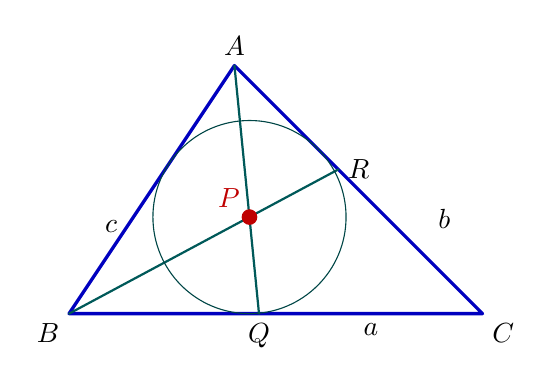
\begin{tikzpicture}[scale=1.05, line cap=round, line join=round]
    \coordinate (A) at (2,3);
    \coordinate (B) at (0,0);
    \coordinate (C) at (5,0);
    \coordinate (Q) at (2.297,0);
    \coordinate (R) at (3.256,1.744);
    \coordinate (P) at (2.182,1.168);
    \draw[blue!75!black, very thick] (A)--(B)--(C)--cycle;
    \draw[teal!70!black, thick] (A)--(Q) (B)--(R);
    \draw[teal!55!black, thin] (P) circle[radius=1.168];
    \node[circle, fill=red!75!black, inner sep=2pt] at (P) {};
    \node[above] at (A) {$A$};
    \node[below left] at (B) {$B$};
    \node[below right] at (C) {$C$};
    \node[below] at (Q) {$Q$};
    \node[right] at (R) {$R$};
    \node[above left, red!75!black] at (P) {$P$};
    \node[below] at (3.65,0) {$a$};
    \node[right] at (4.35,1.15) {$b$};
    \node[left] at (0.7,1.05) {$c$};
  \end{tikzpicture}
  \caption{角の二等分線 $AQ,BR$ の交点にある内心 $P$}
\end{figure}

$AP$と$BC$の交点$Q$, $BP$と$AC$の交点$R$とする．
題意より点$P$が三角形$ABC$の内心だから，$\angle BAQ=\angle CAQ, \angle ABR=\angle CBR$が成り立つ．従って点$X$に対し$\overrightarrow{AX} = \vec{x}$とおくと
\begin{align}
  \begin{cases}
    \vec{q} = \dfrac{b}{b+c} \vec{b} + \dfrac{c}{b+c} \vec{c} \\
    \vec{r} = \dfrac{c}{a+c} \vec{c}
  \end{cases} \label{eq:3}
\end{align}
が成り立つ．点$P$は$AQ, BR$上の点だから $k, l \in \mathbb{R}$として
\begin{align}
  \vec{p} &= k\vec{q} = (1-l)\vec{b} + l\vec{r} \\
  \therefore
  \vec{p}
  &= k \left( \dfrac{b}{b+c} \vec{b} + \dfrac{c}{b+c} \vec{c} \right) \\
  &= (1-l) \vec{b} + l \dfrac{c}{a+c} \vec{c} \quad (\because\text{\cref{eq:3}})\label{eq:4}
\end{align}
と書ける．

(1)と同様にして，$\vec{b} \not\parallel \vec{c}$の時，$u \vec{b} + v \vec{c} = 0 \iff u = v = 0$だから，\cref{eq:4}で係数を比較して
\begin{align}
  \begin{cases}
    1-l = k \dfrac{b}{b+c} \\
    l \dfrac{c}{a+c} = k \dfrac{c}{b+c}
  \end{cases}
  \therefore
  \begin{cases}
    k = \dfrac{b+c}{a+b+c} \\
    l = \dfrac{a+c}{a+b+c}
  \end{cases} \label{eq:5}
\end{align}
である．\cref{eq:4}に代入して整理して
\begin{align}
  \vec{p} = \dfrac{b}{a+b+c} \vec{b} + \dfrac{c}{a+b+c} \vec{c}
\end{align}
だから，
\begin{align}
  \overrightarrow{OP}
  & = \overrightarrow{OA} + \overrightarrow{AP} = \overrightarrow{OA} + \dfrac{b}{a+b+c} \overrightarrow{AB} + \dfrac{c}{a+b+c} \overrightarrow{AC} \\
  & = \dfrac{1}{a+b+c} (a \overrightarrow{OA} + b \overrightarrow{OB} + c \overrightarrow{OC})
\end{align}
となる．従って(1)と同様に考えて
\begin{align}
  \begin{cases}
    u = \dfrac{a}{a+b+c} \\
    v = \dfrac{b}{a+b+c} \\
    w = \dfrac{c}{a+b+c}
  \end{cases}
\end{align}
である．

\end{document}
